\chapter{Contextualización}
\label{chap:contextualizacion}
\vspace{0.5cm}

%%%%%%%%%%%%%%%%%%%%%%%%%%%%%%%%%%%%%%%%%%%%%%%%%%%%%%%%%%%%%%%%%%%%%%%%%%%%%%%%
% Objetivo: Contar cómo estaba la situación antes de empezar,                  %
%           t0do lo que se hizo para familiarizarse con las tecnologías,       %
%           casarlas, etc.                                                     %
%%%%%%%%%%%%%%%%%%%%%%%%%%%%%%%%%%%%%%%%%%%%%%%%%%%%%%%%%%%%%%%%%%%%%%%%%%%%%%%%

\lettrine{E}{n} este capítulo se introducen los conceptos necesarios para la contextualización del trabajo. Se hablará sobre el proyecto D.R.E.A.M.\cite{dream_project} en el que se enmarca el proyecto ROBOBO, y sobre el trabajo previo en el robot.


\section{Proyecto D.R.E.A.M.}
\label{sec:dreamproyect}
%todo Pedir info sobre esto (Dream)
Este trabajo fin de grado se enmarca dentro del proyecto europeo de investigación DREAM (Deferred Restructuring of Experience in Autonomous Machines) que se lleva a cabo en el Grupo Integrado de Ingeniería (GII). El objetivo global de dicho proyecto consiste en el desarrollo de una arquitectura cognitiva que permita a los dispositivos robóticos realizar tareas de aprendizaje y optimización de sus comportamientos. En particular, estas tareas se realizarán tanto durante el período de actividad como durante el período de inactividad de los robots (aprendizaje en fase de sueño) en analogía al funcionamiento del cerebro en lo seres humanos durante los períodos de sueño.

\section{Plataforma ROBOBO 2.0}
\label{sec:roboboplatform}

\begin{figure}
	\centering
	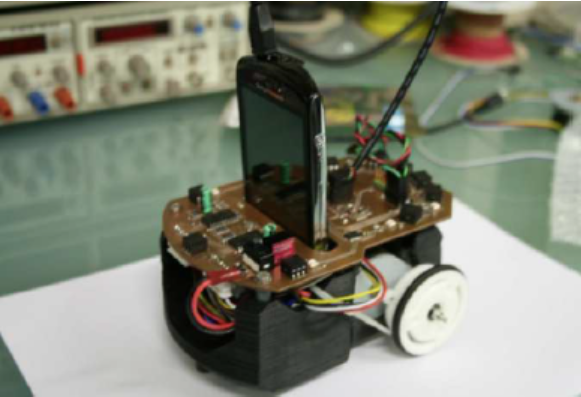
\includegraphics[width=0.8\linewidth]{imagenes/robobo1_0.PNG}
	\caption{Robobo 1.0}
	\label{fig:robobo_1_0}
\end{figure}

La primera versión de la plataforma fue desarrollada por el Grupo Integrado de Ingeniería de la UDC, el ROBOBO 1.0 (Figura \ref{fig:robobo_1_0}) , sirvió como versión conceptual para comprobar la viabilidad del sistema plataforma + smartphone, y presentaba las siguientes características:

\begin{itemize}

	\item 9 LEDs (diodos emisores de luz) RGB para interactuar con el usuario, que cambiaban de color con la proximidad de objetos.
	\item 9 sensores IR de proximidad para proporcionar capacidad de movimiento autónomo: 2 en la parte frontal, 4 en los laterales y los últimos tres en la parte trasera; de manera que proporcionaba una visión general del entorno.
	\item 2 motores paso a paso (convierten impulsos eléctricos en desplazamientos angulares discretos, es decir, pueden avanzar un ángulo concreto en función de la señal recibida) que aplicaban movimiento a las ruedas, con un paso de 1/8, con gran precisión de giro.
	\item Compatibilidad con dispositivos Android.
	\item Capacidad de interacción con otros dispositivos ROS.
	\item Conexión USB para la comunicación con el teléfono inteligente.

\end{itemize}


\begin{figure}
	\centering
	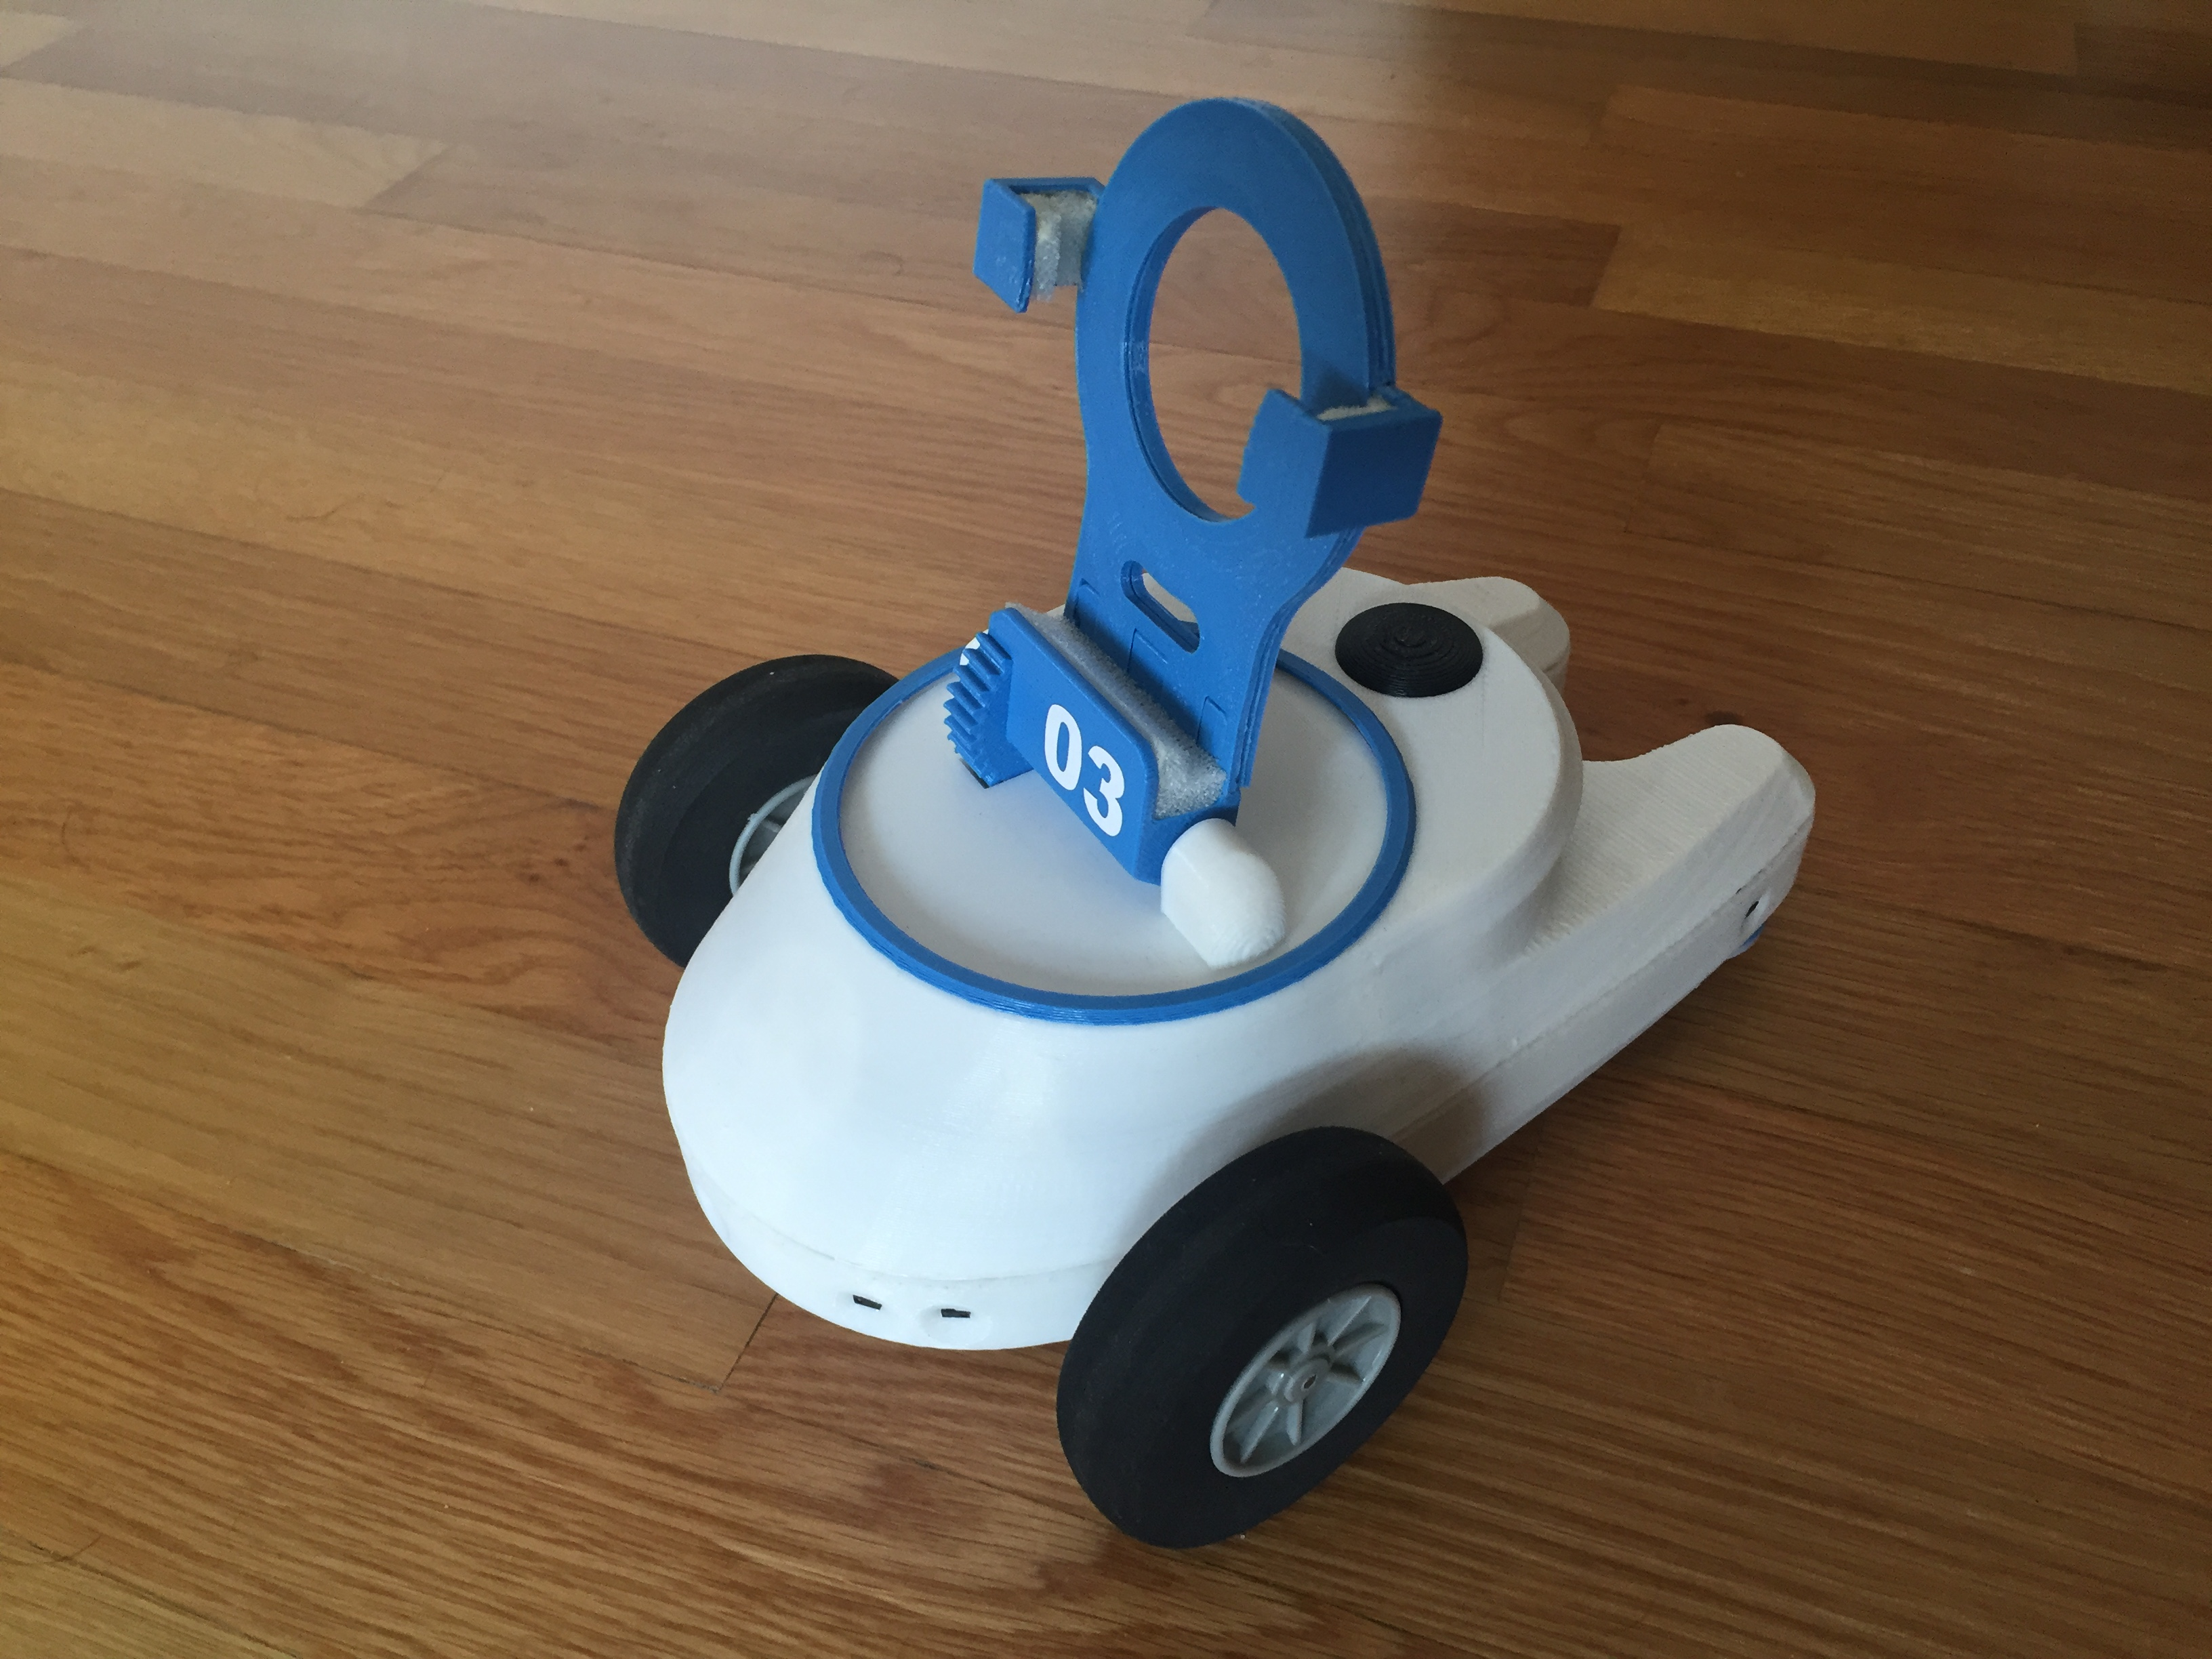
\includegraphics[width=0.8\linewidth]{imagenes/robobo_rob.JPG}
	\caption{Robobo 2.0}
	\label{fig:robobo_2_0}
\end{figure} 

La segunda versión, el ROBOBO 2.0 (figura \ref{fig:robobo_2_0}) , fue desarrollada para solventar las carencias de la primera versión y añadir ciertas mejoras. Tras este rediseño, las características del robot pasaron a ser:

\begin{itemize}
	\item LEDs: pasan a ser 21, 9 de ellos formando una matriz de comunicación para dar una información avanzada mediante colores y formas.
	\item Motores de las ruedas: Pasan a ser motores de corriente continua, menos voluminosos y más eficientes energéticamente. Cada motor cuenta con un encoder magnético, que transforma el movimiento del motor en pulsos eléctricos, que pueden ser interpretados por la parte software del robot.
	\item Comunicación: Se elimina la comunicación USB a favor de una conexión Bluetooth, lo cual permite utilizar diferentes smartphones con distintas posiciones de los puertos.
	\item Plataforma universal para smartphones: Se incluye un adaptador universal para teléfonos moviles, montado sobre una plataforma motorizada que permite el movimiento del snartphone sobre el chasis del robot. Esta plataforma tiene dos grados de libertad, rotación e inclinación.
	\item Sensores: Modificadas tanto el tipo, la cantidad y la posición. Se colocaron en la siguiente disposición (figura \ref{fig:robobo_2_0_sensors}):
	\item \begin{figure}
	\centering
	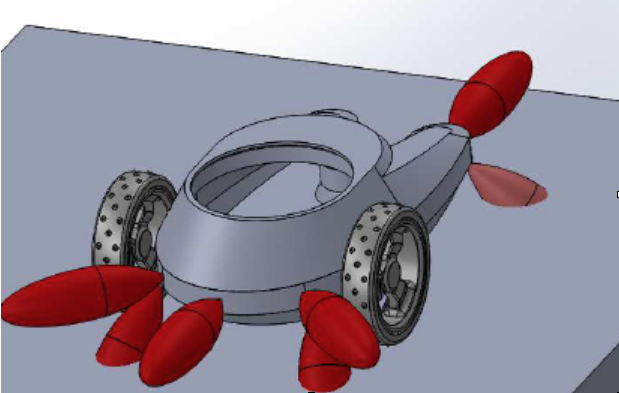
\includegraphics[width=0.8\linewidth]{imagenes/robobo_2_sensors.png}
	\caption{Disposición de los sensores en el ROBOBO 2.0}
	\label{fig:robobo_2_0_sensors}
\end{figure} 
	\begin{itemize}
	\item 3 sensores para la detección de colisiones en la parte delantera; uno frontal y los otros dos cercanos a las ruedas, de tal forma que el ROBOBO no pudiera chocar, frontalmente con ninguna superficie.
	\item 2 sensores inclinados hacia abajo para la detección de caídas, en la parte delantera, colocados cerca de las ruedas, es decir, la zona con mayor peligro de caídas.
	\item 2 sensores de caídas y 2 de colisiones, de forma similar a los anteriores, en la zona anterior del robot. 
	
	\end{itemize}
	\item Unión sensores-microcontrolador: se han cambiado las resistencias pull-up anteriores por un multiplexor. Se consigue, así, un único elemento de muchas entradas y una única salida capaz de permitir la transmisión de una, y solo una, de las entradas hacia la salida.

	\item Microcontrolador: PIC32MX534F064H, de la familia de microcontroladores de 32 bits, económico, con alta capacidad de procesamiento, diversidad de interfaces de comunicación y multitud de puertos de entrada y salida; además de que su entorno de desarrollo y su compilador son gratuitos. Este microcontrolador se programa mediante el protocolo de comunicación I2C y logra el contacto entre sensores y microcontrolador mediante buses línea de reloj “SCL” y buses línea de datos “SDA”.




\end{itemize}




\subsection{ROBOBO! Framework}

\begin{figure}
	\centering
	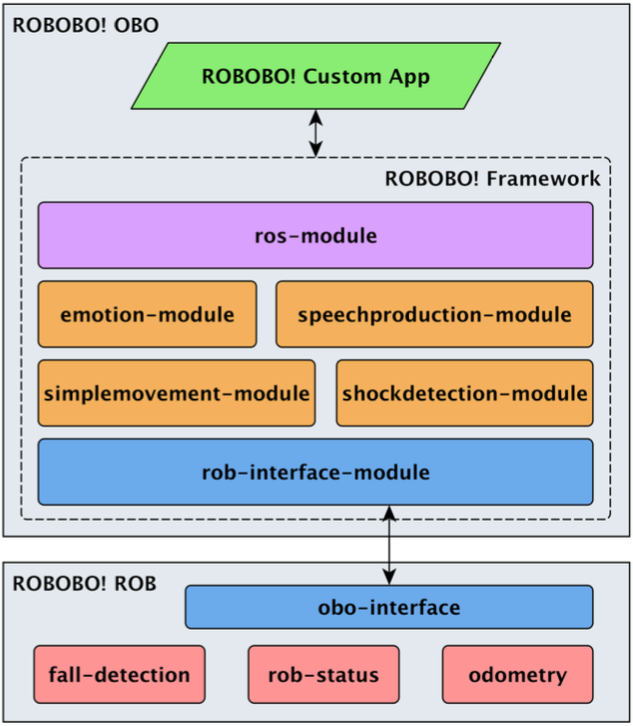
\includegraphics[width=0.6\linewidth]{imagenes/robobo_framework.png}
	\caption{Estructura de ROBOBO! framework dentro del entorno ROBOBO}
	\label{fig:robobo_framework_estructure}
\end{figure}

El ROBOBO! Framework\cite{RoboboFramework} es el framework de desarrollo usado para desarrollas aplicaciones para el ROBOBO. Está diseñado de manera modular, de forma que facilita la extensión del mismo con nuevos módulos. Está publicado con una licencia libre LGPL v3.
Ofrece el módulo \textit{rob-interface-module}, que permite la comunicación entre la plataforma robotizada (denominada ROB, figura \ref{fig:robobo_2_0}) y el smartphone (denominado OBO en el sistema). También proporciona el módulo \textit{ros-module} que sirve de interfaz entre el robot y ROS \cite{Ros}.











 